# A Case Study: Light-Weight Relevance Filtering for Research Papers

\subsection*{The relevance problem}

Modern AI systems increasingly use Retrieval-Augmented
Generation (RAG)~\cite{lewis2020retrieval} to answer questions
about large document collections. RAG has two halves: (a) an
{\em embedding} stage that finds relevant documents, and (b) a
{\em generation} stage where an LLM synthesizes an answer from
those documents. The first half is itself a classical problem:
given a query and a corpus of thousands or millions of
documents, return only those that are relevant. Most modern
implementations solve this with dense vector embeddings from
deep neural models (BERT, OpenAI's \texttt{text-embedding-3},
sentence-transformers, etc.).

But before embedding RAGs there were active learners. In 2018,
Yu et al.~\cite{yu2018finding} studied this problem in a
particularly painful instance: {\em primary study selection}
for systematic literature reviews (SLRs) in software
engineering. An SLR conductor starts with a search query
returning thousands of candidate papers, of which a few dozen
are actually relevant. Reading every candidate takes weeks
or months~\cite{kitchenham2010,carver2013}. Yu et al.\ asked
whether active learning could reduce that cost.

Yu's approach, called FASTREAD, sat on top of three building
blocks: a linear SVM, an active acquisition strategy
(uncertainty sampling early, certainty sampling later), and
aggressive undersampling for class balance. After reviewing
$\sim$300--800 papers from corpora of 1{,}700--8{,}900,
FASTREAD recovered 95\% of the relevant ones. That is a
20--50\% reduction over the previous state of the art from
medicine and legal e-discovery~\cite{wallace2010,miwa2014,
cormack2014}.

\subsection*{An EZR replication, with TWCNB instead of SVM}

Yu's tool used SVMs. We asked: can EZR's substrate, plus
TWCNB (Rennie et al., ICML 2003~\cite{rennie2003}), do the
same thing? TWCNB (Transformed Weight-normalized Complement
Naive Bayes) is the four-trick refinement of Naive Bayes that
closed the gap to SVMs on text classification:
\begin{enumerate}
\item Estimate per-word weights from each class's
{\em complement} (all rows {\em not} in that class),
not the class itself. This corrects bias from skewed class
sizes---which is severe here, where ``relevant'' is 1--2\% of
the corpus.
\item L1-normalize the per-class weight vectors so classes
with strong word dependencies do not dominate.
\item Replace raw term frequencies with $\log(1+f)$, since
real text follows a power-law (``bursty'') distribution, not
a multinomial.
\item Down-weight common terms by inverse document frequency.
\end{enumerate}
The four tricks decompose into named pieces---\textsf{idfs},
\textsf{counts}, \textsf{weights}---each of which is small.
The full implementation (above) is around 30 lines, riding on
the \cls{Data}/\cls{Sym}/\cls{Num} substrate already in EZR.

\subsection*{Data and metrics}

We use Yu's four corpora, each derived from a published SE
SLR by reverse-engineering the search query and final
inclusion list (see Yu's Table~1, reproduced here as
Table~\ref{slr}). The datasets are named after the lead
authors of the source SLRs: Hall et al.~\cite{hall2012} on
fault prediction, Wahono~\cite{wahono2015} on defect
prediction, Radjenovi\'c et al.~\cite{radjenovic2013} on
software fault metrics, and Kitchenham et al.\
\cite{kitchenham2010} on a tertiary review.

\begin{table}[!t]
\caption{The four SLR corpora from Yu et al.\
\cite{yu2018finding}. Each is a search-engine query result
where a small minority of candidates are relevant.
Kitchenham has two relevance levels: 132 papers relevant by
title/abstract, of which 45 survive content review.}
\label{slr}
\begin{center}
\footnotesize
\begin{tabular}{lrr}
\hline
Dataset & \#Candidate & \#Relevant \\
\hline
Wahono       & 7002 & 62 \\
Hall         & 8911 & 104 \\
Radjenovi\'c & 6000 & 48 \\
Kitchenham   & 1704 & 45 (132) \\
\hline
\end{tabular}
\end{center}
\end{table}

We use two metrics from the IR literature, both standard:

\begin{itemize}
\item {\em Recall} $= \mathit{tp} / (\mathit{tp} +
\mathit{fn})$: the fraction of truly relevant papers that
were correctly retrieved. Higher is better. The Yu-style
target is 95\% recall.
\item {\em False alarm} (also called {\em pf}, false-positive
rate) $= \mathit{fp} / (\mathit{fp} + \mathit{tn})$: the
fraction of {\em irrelevant} papers that were incorrectly
returned as relevant. Lower is better.
\end{itemize}
Yu's paper reported only recall; reporting recall alone hides
how much {\em irrelevant} reading the user must still do.
Reporting both is the right protocol.

\subsection*{Experimental rig}

For each dataset, we warm-start with 25 randomly drawn rows
(both classes), train TWCNB, and then add one row at a time
chosen by {\em certainty sampling} (the unlabeled row TWCNB
ranks most strongly as ``yes''). After each label, we retrain
and re-score. We report median and IQR over 20 repeats.
Acquisition stops when 95\% recall is reached or the budget
is exhausted.

We ran this in two configurations:
\begin{itemize}
\item {\bf Non-normalized}: skip Rennie's L1 normalization
(Rennie's trick \#2). All other tricks remain.
\item {\bf Normalized}: include the L1 normalization, exactly
as the TWCNB paper recommends.
\end{itemize}

\subsection*{Results}

Figure~\ref{slrfig} shows recall and false alarm for both
configurations on all four datasets.

\begin{figure*}[!t]
\centering
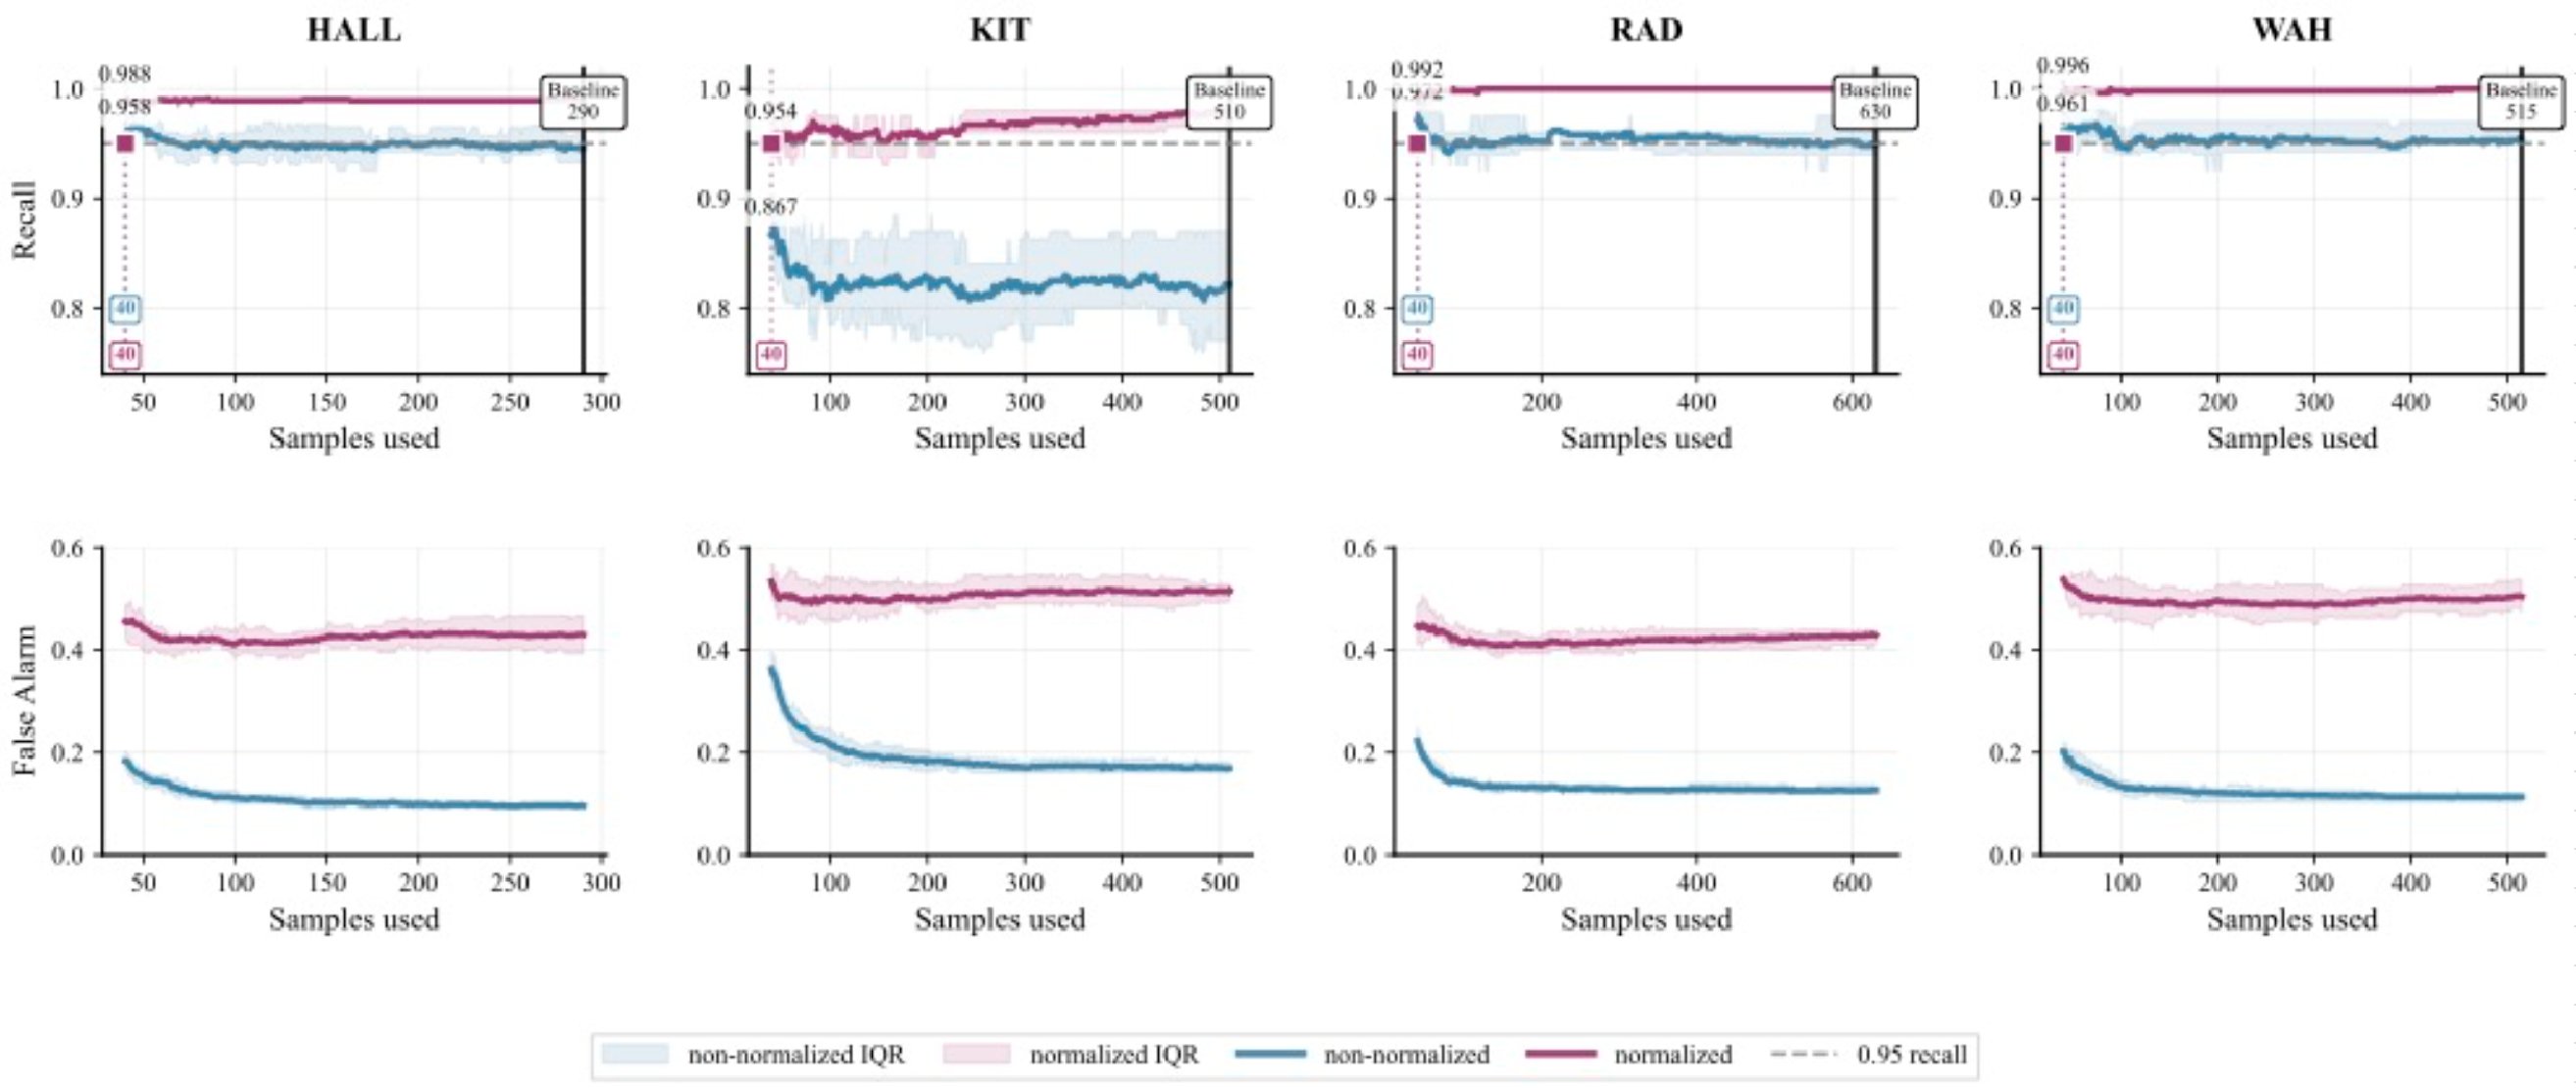
\includegraphics[width=\linewidth]{kit.pdf}
\caption{Recall (top) and false alarm (bottom) as a function
of labels acquired, for non-normalized TWCNB (blue) and
normalized TWCNB (red). Warm start = 25; each curve is the
median over 20 repeats with shaded IQR. Vertical bars mark
the labeling budget at which Yu et al.~\cite{yu2018finding}
reached the same recall with FASTREAD; numerical labels at
left mark the recall after the warm start.}
\label{slrfig}
\end{figure*}

Three things stand out.

{\em First}, on three of the four corpora (Hall,
Radjenovi\'c, Wahono), non-normalized TWCNB reaches Yu's
95\% recall {\em immediately after the warm start}. The
recall curves are flat across the entire budget. Forty
labels are enough. This is well below the 290--630 labels
FASTREAD required, which itself was a 20--50\% reduction
over the state-of-the-art SVM methods of its time. The
problem turns out to be substantially easier than Yu's
results suggested.

{\em Second}, normalization (the red lines) helps recall
slightly on some datasets but {\em substantially harms}
false alarm on all of them---non-normalized false alarms
sit at 10--20\% while normalized false alarms sit at
40--50\%. A user following the literal TWCNB recipe would
end up reading 4--5$\times$ as many irrelevant papers as
necessary. Rennie et al.\ recommended L1 normalization to
correct weight-magnitude bias from feature dependencies; on
their text-classification benchmarks (20 Newsgroups, Reuters,
Industry Sector), it helped. On {\em our} relevance-filtering
task, it does not. This is the kind of finding that only
emerges if you re-run the prior work and report metrics the
prior work omitted---in this case, false alarm, which Yu et
al.~\cite{yu2018finding} did not measure.

{\em Third}, the Kitchenham column is the interesting case.
On the strict 45-paper relevance label, recall plateaus at
85\%, well below the 95\% target. But Kitchenham's corpus
has {\em two} relevance levels: 132 papers passed
title/abstract review, of which 45 survived content review.
At 82\% recall on the 132-paper label, TWCNB still finds
roughly 108 relevant papers while missing fewer than 25.
For a researcher whose goal is ``find me dozens of relevant
papers, quickly,'' this is still useful---and, again,
achieved with 40 labels.

\subsection*{The lesson}

This study replicates and extends prior SE work using a
simple method. Compared to Yu's FASTREAD, EZR + TWCNB:
\begin{itemize}
\item uses fewer labels (40 vs.\ 290--630) on three of four
corpora;
\item uses a simpler classifier (Naive Bayes vs.\ linear SVM);
\item uses a smaller codebase (the relevant filtering logic
is around 30 lines of TWCNB plus a small driver, riding on
EZR's existing substrate);
\item reports both recall {\em and} false alarm, surfacing
that one of TWCNB's recommended tricks (normalization) is
counterproductive in this domain---a finding the original
study could not have made without measuring false alarm.
\end{itemize}

This is half of RAG. The first half---finding the relevant
documents in a large corpus---is exactly what active TWCNB
does here, with no embeddings, no neural network, and no
GPU. The second half---generating natural-language answers
from those documents---is where LLMs are genuinely required.
We are not arguing that LLMs are unnecessary; we are arguing
that a non-trivial portion of what RAG pipelines do can be
done by methods that pre-date the deep-learning revolution,
when those methods are built on a substrate that makes them
easy to express.

The risk we want to flag is the inverse of Sutton's bitter
lesson. Sutton warned that researchers cling to clever
hand-crafted methods when scale would do better. The
companion warning, equally important, is that researchers
adopt scale-heavy methods reflexively---reaching for an LLM
and an embedding API for problems where 30 lines of TWCNB
on a 1{,}700-row corpus would suffice. The cognitive bias
toward additive complexity~\cite{Fillon25,adams2021people}
shows up here too: it is easier to add a vector database
than to ask whether one is needed. Trying the simple thing
first costs almost nothing and, occasionally, ends the
investigation.

\appendix
\section*{Building and Displaying Trees}
# Tree Growth and Use

EZR's regression trees are built {\em after} active learning is done.
The {\em best}/{\em rest} machinery in \textsf{acquire} (line~\ref{s1})
collected a small set of labeled rows; \textsf{treeGrow} now distills
those rows into a readable rule set that predicts \textsf{disty}.

A \cls{Tree} node holds the rows that fell to it (in a child \cls{Data}
called \textsf{d}), a summary \cls{Num} of their \textsf{disty} values
(\textsf{ynum}), and---if the node has split---the chosen column,
cut value, and two children:
\begin{minted}{python}
class Tree: 
  def __init__(i, data, rows):
    i.d = clone(data, rows)
    i.ynum=adds((disty(data,row) for row in rows),Num())
    i.col,i.cut = None,0
    i.left=i.right=None
\end{minted}
\textsf{treeCuts} proposes split points for one column. For symbols,
all distinct values are candidates; for numbers, just the median (a
deliberate simplification that keeps trees small and fast):
\begin{minted}{python}
def treeCuts(col, rows): 
  vs=[row[col.at] for row in rows if row[col.at]!="?"]
  if not vs: return []
  return (set(vs) if Sym == type(col)
          else [sorted(vs)[len(vs)//2]])
\end{minted}

\textsf{treeSplit} evaluates one (column, cut) pair by partitioning
the rows and scoring the result by weighted \textsf{spread} of
\textsf{disty}---the same \textsf{spread} function defined earlier
(standard deviation for \cls{Num}s, entropy for \cls{Sym}s). Lower
scores mean tighter, more predictable leaves:
\begin{minted}{python}
def treeSplit(data, col, cut, rows): 
  l_rows,r_rows,l_num,r_num=[],[],Num(),Num()
  for row in rows:
    v = row[col.at]
    go=v=="?" or (v==cut if Sym==type(col) else v<=cut)
    (l_rows if go else r_rows).append(row)
    add(l_num if go else r_num,disty(data,row))
  s=l_num.n*spread(l_num)+r_num.n*spread(r_num)
  return s,col,cut,l_rows,r_rows
\end{minted}

\textsf{treeGrow} ties it together: enumerate every (column, cut)
pair from the $x$ columns, keep splits where both sides have at
least \textsf{the.learn.leaf} rows, take the lowest-spread split,
and recurse. The recursion stops when too few rows remain to split
further:
\begin{minted}{python}
def treeGrow(data, rows): 
  tree = Tree(data, rows)
  if len(rows) >= 2 * the.learn.leaf:
    splits = (treeSplit(data, col, cut, rows)
              for col in tree.d.cols.xs
              for cut in treeCuts(col, rows))
    if valid := [s for s in splits
        if min(len(s[3]),len(s[4]))
           >= the.learn.leaf]:
      _, tree.col, tree.cut, left, right = min(
        valid, key=lambda x: x[0])
      tree.left  = treeGrow(data, left)
      tree.right = treeGrow(data, right)
  return tree
\end{minted}

That is the entire builder. Note what is {\em not} here: no entropy
gain, no Gini, no pruning pass, no surrogate splits, no bagging.
\textsf{spread} already handles both numeric and symbolic targets
(by polymorphism on \textsf{col} type), so one routine covers what
CART and C4.5 split into many. The deliberate restriction to the
median cut for numeric columns means \textsf{treeGrow} considers
$O(|\textit{xs}|)$ splits per node rather than $O(|\textit{xs}| \cdot
|\textit{rows}|)$; on the small label sets EZR works with, this is
both fast and surprisingly effective.

\smallskip

Once the tree exists, three small functions use it.
\textsf{treeLeaf} routes a row to its leaf by walking the splits
(missing values fall right, by convention):
\begin{minted}{python}
def treeLeaf(tree, row): 
  if not tree.left: return tree
  v = row[tree.col.at]
  go = v!="?" and (v<=tree.cut
    if Num==type(tree.col) else v==tree.cut)
  return treeLeaf(tree.left if go else tree.right,row)
\end{minted}

\textsf{treeNodes} is a depth-first generator that yields every node
along with its level, the column/op/cut that led to it, and---when a
node has children---visits them sorted by \textsf{mid(ynum)} so that
the most promising branch (lowest \textsf{disty}) is shown first. This
sort is what makes printed trees like Figure~\ref{htree} read
top-to-bottom from best to worst:
\begin{minted}{python}
def treeNodes(tree,lvl=0,col=None,op="",cut=None): 
  yield tree, lvl, col, op, cut
  if tree.col:
    ops=("<=",">") if Num==type(
      tree.col) else ("==","!=")
    kids=sorted([(tree.left,ops[0]),
      (tree.right,ops[1])],
      key=lambda z:mid(z[0].ynum))
    for k, txt in kids:
      if k: yield from treeNodes(k,lvl+1,
        tree.col,txt,tree.cut)
\end{minted}

\textsf{treeShow} consumes that generator to print the tree. Each
line carries the indented split, the leaf's mean \textsf{disty}, the
row count, and the per-goal \textsf{mid} values---which is exactly
the format of Figure~\ref{htree}, where the gap between rows
\rc{1} and \rc{2} revealed the 43\% productivity win:
\begin{minted}{python}
def treeShow(tree): 
  for t1,lvl,col,op,cut in treeNodes(tree):
    p=f"{col.txt} {op} {o(cut)}" if col else ""
    if lvl > 0: p = "|   "*(lvl-1) + p
    g={col.txt:mid(col) for col in t1.d.cols.ys}
    print(f"{p:<{the.show.show}}"
          f",{o(mid(t1.ynum)):>4}"
          f" ,({t1.ynum.n:3}), {o(g)}")
\end{minted}
% Finally, \textsf{treePlan} turns the tree into {\em counterfactual
% advice}. Given the leaf where a row currently sits (\textsf{here}),
% it walks every other leaf and yields those with meaningfully lower
% \textsf{disty}---``meaningfully'' meaning beyond a small-effect
% threshold (Sawilowsky's $0.35\sigma$, the same threshold used in
% \textsf{wins} at line~\ref{wins}). For each such leaf, it reports
% which $x$ columns would need to change and to what:
% \begin{minted}{python}
% def treePlan(tree, here): 
%   eps = the.stats.eps * spread(tree.ynum)
%   for there,_,_,_,_ in treeNodes(tree):
%     if there.col is None and \
%       (dy:=mid(here.ynum)-mid(there.ynum))>eps:
%       diff=[f"{col.txt}={o(mid(col))}"
%         for col,h in zip(there.d.cols.xs,here.d.cols.xs)
%         if mid(col) != mid(h)]
%       if diff:
%         yield dy, mid(there.ynum), diff
% \end{minted}

% This is what makes EZR's trees more than predictors. They are
% {\em advisors}: they not only score a configuration but tell the
% engineer what to change to reach a better one---and silently
% report which $x$ variables never appeared in any split, which is
% how Figure~\ref{used} could conclude that fewer than ten variables
% matter even on 1000-variable data.
\bibliography{bib3,main}
\end{document}
